% CREATED BY DAVID FRISK, 2016
\section{Methods}
This section introduces the methods used throughout this project, along with a description of the tools and setup of the simulations. The approach is to collect data from human movement to use in a pre-evolution. Then use the pre-evolved model when preforming simulations on a Bioloid robot model, and later in the physical robot. Much of the basic simulation enviroment was provided by a previous research project \cite{studentProj}, which was further developed during this project.

%To be able to achive the goal stated in the introduction, the project was devided into sections. First, data was collected from a human during a walking cycle. The collected data were processed to later be used for simulations. The simulations were prepared and then performed. The results from the simulations were then implemented into the bioloid. All of these sections will be described in more detail in this chapter in a chronological order  }

%Skriv intro till kapitlet, typ vår tankegång; samla data, använda data i preprocessing, använda preprocessed modell i simulering, testa simuleringen på robot.

\subsection{Record Physical Model} \label{recordPhysicalModel}

\subsubsection{Data Collection}
%Robot has 18 DoF, divided into 8 joints. Record human data from corresponding joints on human.
%Using mobile phones, easy good accelerometer. LiU sensor fusion, export CSV. Putting phones in socks, taping to joints.

%Recorded walking cycle. Jump before start of each cycle as init signal.

%Gather and assemble hardware needed.
%Setup hardware/software interface to collect data.
%Find ideal amount of sensors and their location.
%Gather movement data.

The Bioloid robot has 18 Degrees of Freedom (DoF), which is divided on 8 different joints. These joints can be seen in Figure \ref{fig:Robot_Joints}. To gather data from a human during a walking cycle, accelerometers were strapped to the human in the joints corresponding to the joints of the Bioloid robot, as seen in Figure \ref{fig:Human_Joints}. Smartphones with the app \textit{Sensor Fusion} \cite{sensorfusion} was used to collect the accelerometer data. Using mobile phones enabled easy access to many high quality sensors, and the app provided an interface to export raw sensor data directly to CSV format. The phones were strapped to the joints shown in Figure \ref{fig:Human_Joints}. A walking cycle was initiated with a jump, to find a clear correlation in initialisation between devices, making it easy to extract and allign the signals. More than one walking cycle was recorded during the same session separated by the initialisation signal.
\begin{figure}[H]
    \centering
    \begin{subfigure}[b]{0.5\textwidth}
        \centering
        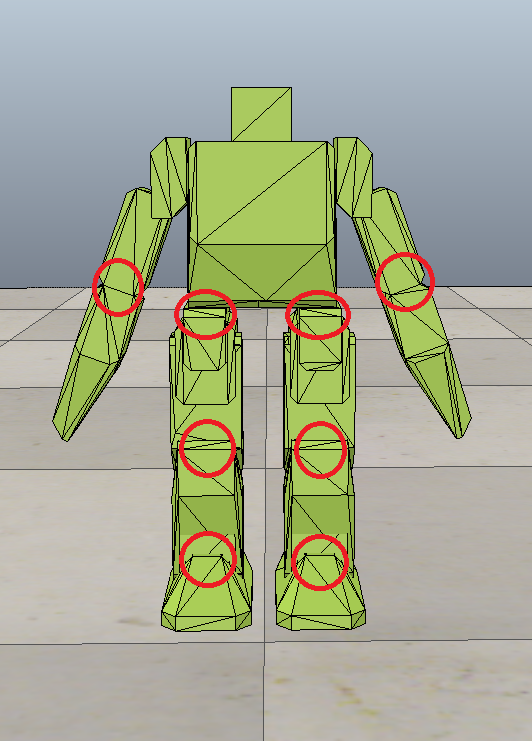
\includegraphics[scale=0.50]{include/figure/Robot_Joints.PNG}
        \caption{Bioloid with joint locations indicated by red circles. }
        \label{fig:Robot_Joints}
    \end{subfigure}%
    ~ 
    \begin{subfigure}[b]{0.5\textwidth}
        \centering
        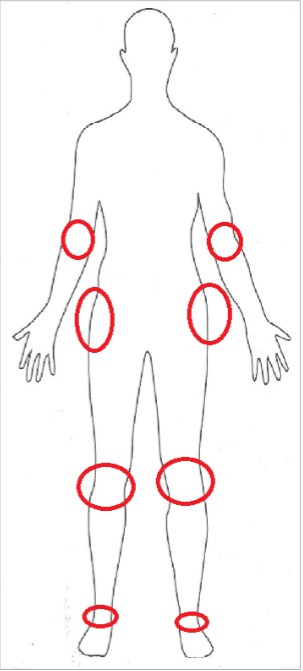
\includegraphics[scale=0.50]{include/figure/Human_Joints.PNG}
        \caption{Human body with accelerometer locations indicated with red circles.}
        \label{fig:Human_Joints}
    \end{subfigure}
    \caption{Joints examined during data collection}
    \label{fig:RLH1}
\end{figure}
\subsubsection{Data Processing}
The recorded data from the walking cycles were processed to align the data between devices and extract walking cycles. All signals were normalised to account for different sensitiveties between sensor models, thus removing bias.


%The X,Y and Z acceleration directions from the joints correkating to the initialization signal were extracted  Once the data was cleared of most noise and the XYZ was extracted, it needed to be normalized because of the fact that the different mobile phones had their differences in the data collected which would lead to bias in the data if not normalized. The results after data collecting and processing was plotted in a graph to give a visual representation, see Figure \ref{fig:AllCyc}   }\\


%Process movement data to be free from noise and possible to use for future steps

%Read recorded data and extract XYZ in joints correlated according to init signals (start at same time). Normalise data to reduce bias from different devices


\subsection{Pre-Evolution}

\subsubsection{Evolve to Fit Physical Model}
%Evolving the mathematical model to fit the physical gathered data 
To leverage the behaviour of humans using the collected data presented in Section \ref{recordPhysicalModel}, a pre-evolution was constructed. The main goal of the pre-evolution was to adopt the output of a CPG network to fit the behaviour of the recorded data. Performing the pre-evolution in an environment not requiring any graphical interface or control of a robot model would hypothetically converge faster then using a full-scale simulation environment. Using an optimised model when performing later simulations on a robot model would then ideally evolve a better behaviour faster.


\subsubsection{Model Construction}
%Model as a CPG using Matsuoka and GA.
The initial intention was to use the same model in the pre-evolution as in the evolution in the robot simulation. But it was discovered that the existing simulation and evolution environment were too highly linked together, meaning that it was easier to construct an independent pre-evolution model. The model was higly inspired by the existing environment, using the Matsuoka model described in \ref{modelOfNeuralOscillator} to model the CPGs and initial parameters as presented in Table \ref{tab:parameters}. The pre-simulation investigated two different types of genomes. In the first case only the connections between the neurons in the CPG network was used, while in the second case all the parameters of the Matsuoka model was used.

The pre-simulation was performed on a CPG network of 18 neurons, corresponding to the 18 DoFs on the humanoid robot. The neurons were initialised fully connected using a connection matrix with random values. The input model by Liu introduced in Section \ref{choiseOfInputToOscillator} was used, the outputs were initiated randomly, since it was required that the output values were initialised to non-zero values to start the evolution. The CPG model was simulated over 20 seconds with a timestep of 0.01 seconds, corresponding to the time of one recorded walking cycle, generating an output signal. The population size was varied between simulations between 20-40 individuals, and full-scale evolutions were made with 500-1000 generations.


\subsubsection{Fitness and Reinforcement}
%Use correlation as fitness functuion. 
When simulated, the CPGs were evaluated by assigning each neuron to a DoF, then comparing the output signal to the corresponding recorded reference signal. This was done by taking the \textit{correlation} between the output signal and the reference signal. A correlation of 1 mean full correlation (identic signals) and a correlation of -1 indicates no correlation (signals shifted half a period). The fitness score was aquired by taking the absolute value of the \textit{lowest} correlation between an output DoF and a reference DoF in an individual, the idea being to maximise the worst correlation in each population. Other fitness functions can be imagined as measuring different similarities between the signals, analysing the moments of the correlation distribution, analysing symmetry between signals, evaluting each DoF individually instead of depending on the rest of the individual, etc. 

Once evaluated, the next generation was chosen by tournament selection, with a tournament size of a fifth of the population size. Elitism was implemented not to loose the best individual, mutations and permutations were randomly applied to the rest of the population. 

\subsection{Implementation of the GA and Simulation}
The method used to evaluate and iterate the weights for the CPG was a standard genetic algorithm, with elitism, tournament selection, mutations and crossovers. The specific parameters of the model can bee seen in Appendix \ref{app:GAparametersPrimary}. The fitness of each individual was evaluated by measuring the distance a simulated 3D model of the Bioloid could travel. The simulated Bioloid accepted input signals in the same way as the physical one. This made it possible to accurately measure and analyse the movement of the robot without having to connect it to the actual Bioloid, thereby speeding up the simulation and the algorithm. However, it came at the cost of disrepancies between the simulated enviroment and the real world. The chosen simulation environment in this project was V-REP \cite{v-rep}, in which a model of a Bioloid robot was imported. Based on how far the simulated Bioloid was able to walk, each individual was assigned a fitness value and compared to the rest of the evaluated individuals. Several fitness functions were evaluated, and the one found to be the most useful was one that multiplied the greatest distance the robot travelled, with the lowest height of the robot. This was to prevent the robot from falling over while still rewarding behaviour that pushed it forward. However, based on the specifics of the simulation, such as stability and DoF, it could be varied for a more specialised approach, such as simply the distance travelled forward.

\subsubsection{Configuration of V-REP}
V-REP efficiently allowed for the import and simulation of the Bioloid robot. The 3D model of the Bioloid was the same as used in the previous project \cite{studentProj}, and can be viewed in the V-REP enviroment in Figure \ref{fig:freeBioloid}. After loading the model into a specific V-REP scene, the GA automatically sent signals into the simulation as soon as it started. The V-REP platform also allowed for an arbitrary number of joints/servos to be simulated, meaning the algorithm could be focused to generate patterns only for a select number of servos.  
\begin{figure}[htbp]
    \centering
    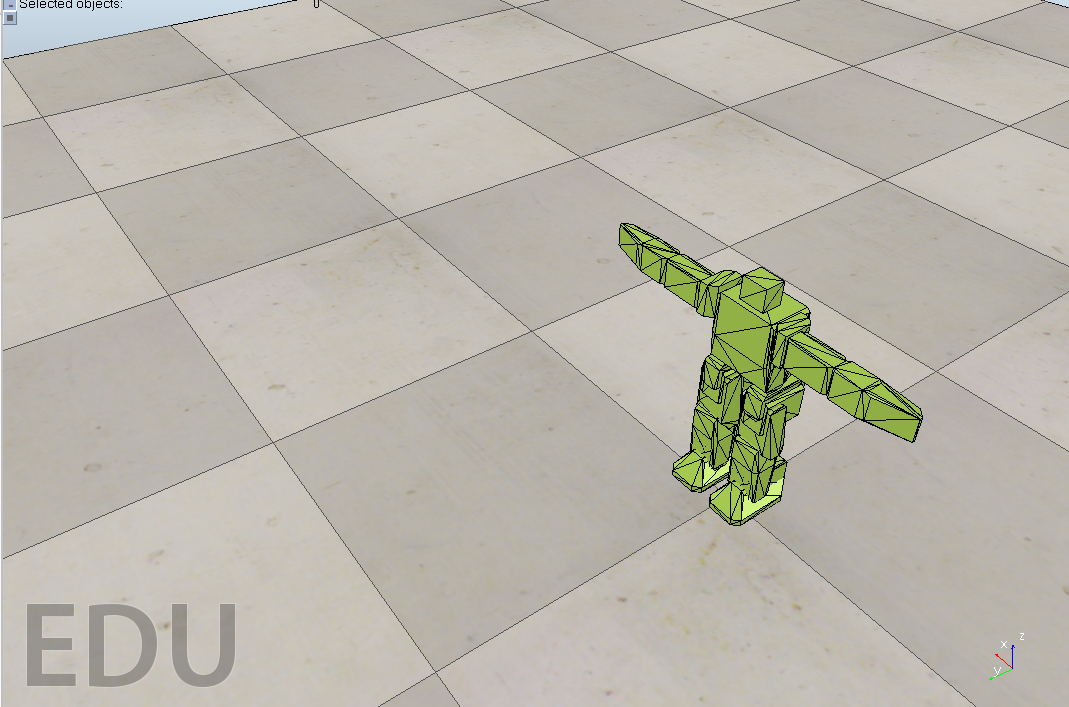
\includegraphics[scale=0.25]{include/figure/freeBioloid.png}
    \caption{The 3D Bioloid model used in the V-REP simulation enviroment.}
    \label{fig:freeBioloid}
\end{figure}
\subsubsection{Physical Implementation and Hardware}
The physical Bioloid robot was pre-assembeled into the standard configuration A \cite{bioloidMan}, offering the highest degree of freedom and replication of the human body. The standard control board on the Bioloid was ignored in favor of connecting directly to the servos and controlling them through an application on the computer. This was accomplished by daisy-chaining all the servos together and connecting them to both a power source and a \textit{USB2Dynamixel} \cite{dongle} dongle, which allows for direct computer-to-servo communication. As before, much of the software infrastructure regarding communication was taken from the previous student project \cite{studentProj}, along with some specific software to communicate with the USB2Dynamixel dongle. As the simulated Bioloid in V-REP had higher friction against its surroundings, the physical Bioloid was modified in order to increase friction of its feet against the floor. This was accomplished with simple modelling clay attached to the soles of its feet.
\subsubsection{Simulation Process}

As previously mentioned, the number of simulated servos could easily be changed in the simulation. Two main approaches were used - one where all 18 joints of the Bioloid were simulated, and one where only 8 were considered. Based on the initial hypothesis, a robot with 18 DoF would be better able to replicate human movement and should thus be able to generate the best results. However, the increased degrees of freedom also led to an increased tendency for the robot to topple and fall. Initially, the simulation with all 18 joints simply let the robot orient itself without any external support and attempt to develop a walking gait from there. It quickly became appearent that the full 18 DoF case would be very slow to develop a walking gait, if it did so at all. In order to speed up the process support rods attached to the robot was used, first four, and then two, in order to prevent the robot from falling down but without interfering too much in the evaluation of the fitness. The 4-rod model can be viewed in Figures \ref{fig:4rods}, and the 2-rod model can be see in Appendix \ref{app:model}, Figure \ref{fig:2rods}. The purpose of these was to take the best result from the simulation with four support rods, and insert that into the simulation with two support rods, and then finally insert the best result from there into a simulation with no support, in order to finally reach a stable gait. 

In the case of only 8 joints, the robot was constricted to only move in the forward direction by means of a support arm, seen in Figure \ref{fig:supportArm}. The arm was used to prevent the robot from falling to either side. The purpose of this was to increase its stability and speed up the simulation, sacrificing freedom of movement and possibly a more human-like gait in order to get stable results faster. Of course, the physical robot would then need to be attached to a support beam as well in this case. Based on preliminary results, the robot was also simulated with all 18 DoF and a support arm, to see if it gave any performance improvements in comparison to the 8 DoF case. Each simulation ran for around 50-70 generations with around 30 individuals in each population. The reasons for these parameters were somewhat arbitrary, as they seemed to give a good enough mix of convergence speed coupled with a reasonable runtime (around 5-7 hours).
\begin{figure}
\centering
\begin{subfigure}{0.5\textwidth}
    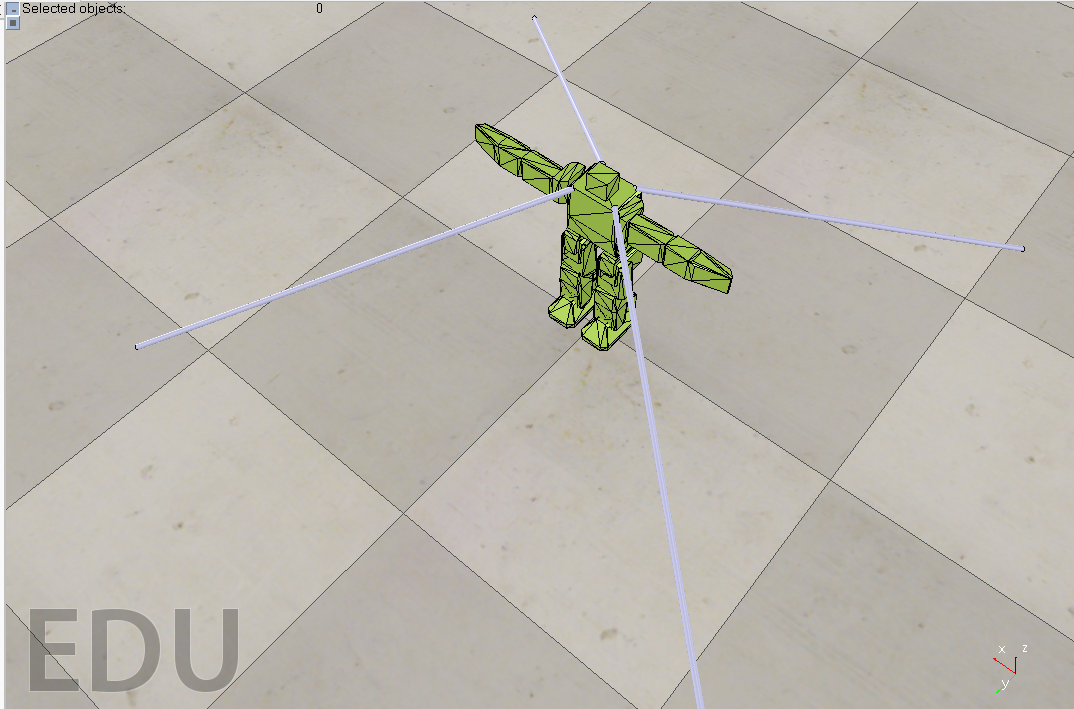
\includegraphics[scale=0.20]{include/figure/4rods.png}
    \caption{The Bioloid model with 4 support arms in the V-REP simulation enviroment.}
    \label{fig:4rods}
    \end{subfigure}
    \begin{subfigure}{0.5\textwidth}
    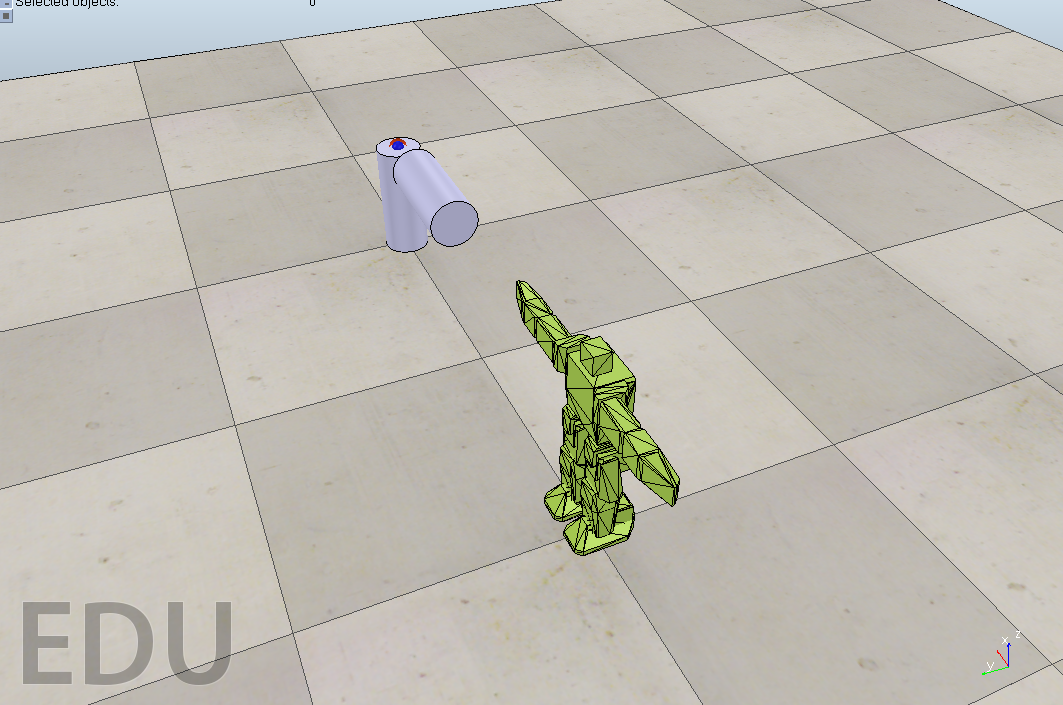
\includegraphics[scale=0.20]{include/figure/supportArm.png}
    \caption{The Bioloid model with the external support arm in the V-REP simulation enviroment.}
    \label{fig:supportArm}
    \end{subfigure}
    \caption{Overview of the different support structures used in the simulation.}
\end{figure}